 ~\vspace{.1in}
 
\section{Modeling with linear equations}

A family with one full-time worker earning minimum wage cannot afford the local fair-market rent for a two-bedroom apartment anywhere in the United States.  
Even families earning above minimum can struggle to rent an apartment for less than 30\% of their income.  As a result, many people need affordable housing.  There are various local, state, and federally funded programs as well as non-profit agencies working to increase availability.

 \hfill \begin{footnotesize} Source:  U.S. Department of Housing and Urban Development \end{footnotesize} % Source used U.S. Department of Housing and Urban Development (HUD) retreived from http://www.hud.gov/offices/cpd/affordablehousing/ on June 20, 2012

In our city there are about \text{64,100} apartments considered affordable.  So the city partnered with local developers to build \text{7,800} more apartments each year.    Our variables are
\begin{center}
\begin{tabular} {l} 
$A=$ affordable housing (apartments) $\sim$ dep \\
$Y=$ time (years from now) $\sim$ indep \\ 
\end{tabular}
\end{center}
Assuming things proceed as planned, after 5 years there would be 
$$\text{64,100 apts } + 5 \text{ years} \ast \frac{\text{7,800 apts}}{\text{year}}=\text{64,100}+\underline{5} \times \text{7,800} =  \text{103,100} \text{ apartments}$$
Generalizing, we get our equation $$\text{64,100}+Y\ast \text{7,800} =  A$$
which can be rewritten as $$A = \text{64,100} + \text{7,800}Y$$
This equation fits our template for a linear equation 
$$\text{dep }=\text{ start } + \text{slope} \ast {\text{indep}}$$

Quick recap.  A function is \textbf{linear} if its graph is a line, and \textbf{nonlinear} otherwise.  The rate of change measures the steepness of the graph for any function, but a line is the same steepness everywhere, so the rate of change, or \textbf{slope} of a line is constant.   Our example is linear because the slope of \text{7,800} apartments per year is constant.  Our starting or fixed amount is the \textbf{intercept}.  In our example it's  \text{64,100} apartments.  The dependent variable and the intercept always have the same units -- apartments in our example.  But $$\text{units for slope} =\frac{\text{units for dep}}{\text{units for indep}}$$ so, in our example slope is measured in apartments \emph{per year}.
These units can help you identify the slope and intercept in a story -- so keep a look out.

How many years will it take the city to reach \text{150,000} apartments at this rate?  After ten years, for example, there would still not be enough affordable apartments because $$A = \text{64,100}+\text{7,800} \ast 10 = \text{64,100}+  \text{7,800}\times \underline{10}=  \text{142,100} \text{ apartments}$$
Continuing successive approximation we get
\begin{center}
\begin{tabular} {|c| |c |c |c |c |c|}\hline
$Y$ & 0 & 5 & 10 & 11 & 12\\ \hline
$A$ & \text{64,100} & \text{103,100} & \text{142,100} & \text{149,900} & \text{157,700} \\ \hline
vs.\ \text{150,000}& low & low & low & low& high\\ \hline
\end{tabular}
\end{center}
This city will reach \text{150,000} affordable apartments within 12 years.

Of course, we could solve a linear equation instead.  We want $A=\text{150,000}$.  
Using our equation $A=\text{64,100} + \text{7,800} Y$ we get
$$ \text{64,100} + \text{7,800}Y = \text{150,000}$$
However, since we want \emph{at least} \text{150,000} affordable apartments, an inequality is even better.  Let's practice that.
 $$ \text{64,100} + \text{7,800}Y \ge \text{150,000}$$
 Subtract \text{64,100} from each side to get
  \begin{eqnarray*}
\cancel{\text{64,100}} + \text{7,800}Y & \ge &\text{150,000}  \\
-\cancel{\text{64,100}} \hspace{.6 in} & & -\text{64,100}  \\ % SU awkward to use hspace!
\end{eqnarray*}
\vspace{-.5in} %VSPACE

\noindent which simplifies to $$ \text{7,800}Y\ge \text{85,900}$$
Divide each side by \text{7,800} to get
$$\frac{\cancel{\text{7,800}}~Y}{\cancel{\text{7,800}}} \ge \frac{\text{85,900}}{\text{7,800}}$$
which simplifies to $$Y \ge   \frac{\text{85,900}}{\text{7,800}} = \text{85,900} \div \text{7,800} = 11.0128205...$$
To be sure $Y \ge 11.0128205...$ we need to round up to get $$Y \ge 12$$

Let's confirm our findings on the graph.
\begin{center}
\scalebox {.8} {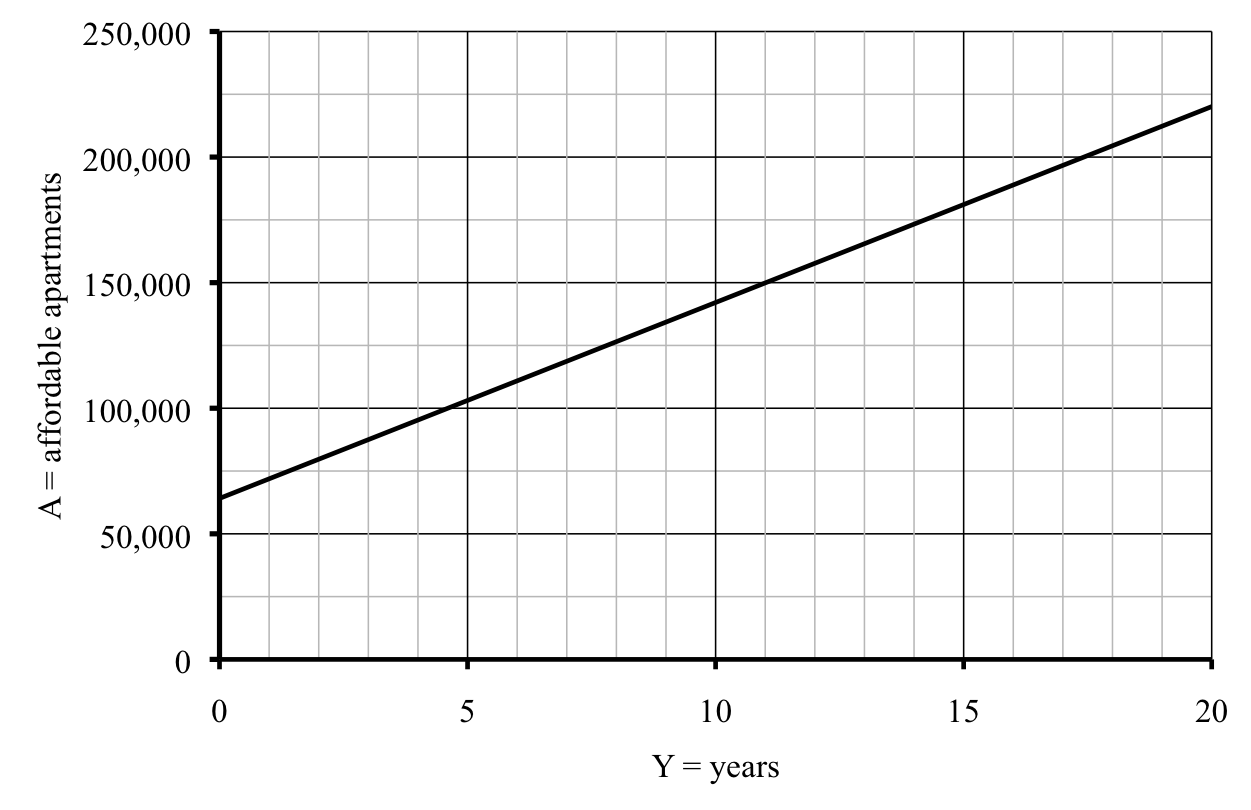
\includegraphics [width = 6in] {apartments.png}}
\end{center}
As expected, the graph is a line.  And we see that the city should reach its goal of \text{150,000} affordable apartments in 12 years, or slightly before then.

 %\section{Modeling with linear equations}

 \begin{center}
\line(1,0){300} %\line(1,0){250}
\end{center}

\section*{Homework}

\noindent \textbf{Start by doing Practice exercises \#1-4 in the workbook.}

\bigskip
 
\noindent \textbf{Do you know \ldots}

\begin{itemize} 
\item What makes a function linear? 
\item What the slope of a linear function means in the story and what it tells us about the graph? 
\item What the intercept of a linear function means in the story and what it tells us about the graph? 
\item The template for a linear equation?  \emph{Ask your instructor if you need to remember the template or if it will be provided during the exam.}
\item How to write a linear equation given the starting amount (intercept) and the rate of change (slope)?   
\item Where the slope and intercept appear in the template of a linear equation? 
\item What the graph of a linear function looks like? 
\item How to solve a linear equation?  
\item Why the rate of change of a linear function is constant?  
\item[~] \textbf{If you're not sure, work the rest of exercises and then return to these questions.  Or, ask your instructor or a classmate for help.} 
\end{itemize}

\subsection*{Exercises}

\begin{enumerate} 
\setcounter{enumi}{4}

\item We looked at the city's plan to increase the number of affordable apartments.  From a current estimate of  64,100  apartments classified as ``affordable,'' they hoped to build 7,800 per year.  At that rate, they can reach a total of 150,000 apartments in 12 years.
\begin{enumerate}
\item Things change.  Revised estimates call for only 6,200 new apartments each year.  At that rate, when will the city reach the 150,000 apartments goal?  Using the same variables as in this section, set up and solve an equation.
\item More bad news.  The definition of ``affordable'' has changed again, so the new count shows only 48,700 apartments on the list.  And still only 6,200 new apartments each year.  Now when will the city reach the 150,000 apartments goal?  Set up and solve an equation.
\item In light of the new definition and, consequently, only 48,700 apartments currently on the list, the city has received additional funding to up the number of apartments built each year.  They would like to return to their goal of having 150,000 affordable apartments in 12 years.  How many apartments do they need to add each year to reach that goal?  Figure out the answer however you like, but check that it works.
\end{enumerate}

\item At a local \textbf{state university}, the tuition each student pays is based on the number of credit hours that student takes plus fees.  The university charges \$870 per credit hour plus a \$560 fee.  The fee is paid once regardless of how many credits are taken.
\begin{enumerate}
\item Name the variables and write an equation relating them.  
\item Find the slope and intercept and explain what each means in terms of the story. 
\item Make a table of values showing the tuition cost for 3 credits, 12 credits, or 16 credits.  
\end{enumerate}
At the local \textbf{community college}, the tuition each student pays is based only on the number of credits.  The college charges \$415 per credit.  
\begin{enumerate}
\item [(d)] Using the same variables as before, write an equation relating them for the community college. 
\item [(e)] Find the slope and intercept and explain what each means in terms of the story. 
\item [(f)] Make a table of values showing the tuition cost for 3 credits, 12 credits, or 16 credits. 
\item [(g)] Graph both functions on the same axes.  
\item [(h)] What do you notice about the graph that confirms the community college is always cheaper?
\end{enumerate} 

\item  Can you tell from the table which of these functions is linear?  Use the rate of change to help you decide.  Remember that numbers may have been rounded.

\begin{enumerate}
\item Ahmed's virburnum shrub. \hfill \emph{Story also appears in 4.2 \#3}

\begin{tabular} {|l|r|r|r|r|} \hline
Week  & 0 & 6 & 10 & 18 \\ \hline
Height (inches) & 16.9 & 19.3 & 20.9 & 24.1  \\ \hline
\end{tabular} \bigskip

\item Rose gold \hfill \emph{Story also appears in 2.3 \#2} 

\begin{tabular} {|c| |c |c  |c |c |c |c |c|}\hline
Grams of gold added & 0 & 0.4 & 0.8  & 1.4 & 1.6  \\ \hline
Percent gold in alloy &50.0 & 58.3& 64.3 & 70.6&72.2 \\ \hline
\end{tabular} \bigskip

\item Sea-ice (in millions of square miles) % This is now on the practice exam.  OK

\begin{tabular} {|c| |c |c  |c |c |}\hline
Year & 1980 & 1990 & 2000 & 2012 \\ \hline
Sea-ice & 3.10 & 2.66 & 2.23 & 1.70 \\ \hline
\end{tabular} \bigskip

\item Wild rice \hfill \emph{Story also appears in 4.5 Exercises}

\emph{Hint:  rewrite the table in order by temperature first.}

\begin{tabular} {|c|| c|c |c|c|c|c|}  \hline
Temperature ($^\circ$F) & 39 & 42 & 41 & 35 & 47 & 45 
 \\ \hline
Acres & 2,300 & 1,950 & 1,425 & 2,015 & 1,233 & 1,256  \\ \hline
\end{tabular} \bigskip

\end{enumerate} 

\item  The temperature was 40 degrees at noon yesterday but it dropped 3 degrees an hour in the afternoon.  Earlier we found the temperature, $T^\circ$F depends on the time, $H$ hours after noon according to the equation 
$$T=40-3H$$
\hfill \emph{Story also appears in 1.1 and 1.2 Exercises}
\begin{enumerate}
 \item When does the temperature drop below freezing (32$^{\circ}$ F)?  Set up and solve the relevant inequality.  Report your answer as an actual time (to the minute) 
 \item When does the temperature drop below zero (0$^{\circ}$ F)? Same instructions. 
 \end{enumerate} 

\item Shanille is collecting rare books.  She inherited 382 books and buys another 3 books every month.
\begin{enumerate}
\item Make a table showing the number of rare books in Shanille's collection at the start, after 1 month, after 12 months, and after 3 years.
\item Name the variables and write an equation relating them.
\item Solve your equation to determine when Shanille will reach her goal of 1,000 rare books.
\item Graph and check.  
\end{enumerate}

\end{enumerate}

